\pdfoutput=1
% !TeX TS-program = Pdflatex
% !TeX encoding = UTF-8 Unicode
% !TeX spellcheck = en
% !BIB TS-program = bibtex
% -*- coding: UTF-8; -*-
% vim: set fenc=utf-8
% Reviewer comments

% Reviewer #1
% Spiking neural networks can produce a very large variety of spiking motifs, and especially so when delays are used. To compute with such motifs, it is necessary to detect them. The detection of spike train can be done using methods spike distances. These methods exists in cases such as Poisson spike train or synchronous spiking, but not for polychronous spiking. This paper presents a method to accurately detect spatio-temporal spiking motifs using a HD-SNN. The paper is interesting, well written in parts but confusing and under explained in others. The motivation of the proposed methods needs to be completed. Why can't one simply use a linear readout (à la liquid state machine) to detect the motif? How about spiking EM approaches (Nessler et al). Do these methods underperform in the experiments considered in the results? The optimization of synaptic parameters to produce a target spike train using a generative model has been studied in the past (Pfister et al 2006, Brea et al. 2006). It would be beneficial to understand the relationship with that work. The mathematical formalism seems to be similar. The derivation is not self-explanatory. Intuitively, one expects that the spiking dynamics, such as threshold and leak should have an impact on the spiking probability, but these are not present in the equation for p(a,t). More explanation on how this result is obtained is necessary to clarify the paper. In the discussion, the statement that the method was applied on "on realistic data" is not true. The data used is synthetic data. How does the method here compare to others in solving recognition/classification/regression problems used in SNN benchmarks? I find the terminology "raster plot" confusing and not helpful because it involves a graphical representation which has little to do with the mathematical optimization.

% Reviewer #2
% The author presents a method for generating and detecting spike-time motifs in synthetic spike rasters of neural activity. Their approach is based on a one-layer feed-forward spiking neural network with synaptic delays. The author randomly builds a generative model for motifs by choosing a random sparse kernel K, which defines motifs as weighted delays from a set of presynaptic spiking neurons. They use this kernel to generate synthetic spike rasters with multiple temporally-overlapping motifs present in each raster. Based on the known kernel K, they invert the kernel to obtain a detection model for the motifs. Presynaptic events are treated as weighted delayed inputs to a "motif" evidence detection neuron for each motif, which can be thresholded to detect the presence of a spiking motif. The author finally randomises the detection kernel and recovers this using gradient-descent optimisation, when the identity and timing of motifs are known and labelled. --- The author identifies my main concern in the perspectives section — as it stands, this model is insufficient to use on real-world experimental data. Nevertheless the author's approach is interesting, and extension to a task more closely approximating real-world use would be very useful. Some additional comments: * It is not explicit what neuron model (or temporal kernel) the author uses. Perhaps I missed this, but exactly how are the elements in kernel K generated (Fig 2b)? There appear to be complex constraints on temporally-related hyper- and de-polarisation effects which I can't see described in the text. * The relationship between Fig 2c and d is difficult to discern, due to the multiplexed motifs. Perhaps the onset of each motif could also be marked in 2d? * It would be interesting to know how robust the detection process is to spiking noise / jitter in synthetic rasters. The author mentions temporal dithering / jitter in the introduction, but the evaluation of the approach is only performed in the noiseless case. * In Results (p7 and Fig 3), the accuracy / "correct detection" metric is not precisely defined. Is this sensitivity per time bin? This should be defined concretely. * For Fig3c, the correlation metric should be defined clearly, and results should be stated numerically in the text. The author states that "all kernels were correctly recovered", but Fig 3c shows several off-diagonal correlation elements with large values.

% Reviewer #3
% While I am not a expert in this particular application, the paper reads well and the mathematics are sound. I would miss more on the motivational side apart from scaling. What are those spiking motifs, what is the impact of being able to detect them, what offers to the neuroscience community? Furthermore, while there is little mention for the causes of these patterns, it could be interesting to relate it (this is just a suggestion) to the spiking coding network theory that posses that the neurons coordinate to have an efficient population coding. See: - Perception: Denève, S., & Machens, C. K. (2016). Efficient codes and balanced networks. Nature neuroscience, 19(3), 375-382. - Motor control: Slijkhuis, F. S., Keemink, S. W., & Lanillos, P. (2022). Closed-form control with spike coding networks. arXiv preprint arXiv:2212.12887. Those are generative models of coordinated spikes that obey prediction error minimization. There are models of those that include delays. Comments - 1.2 Decoding neural activity using spike distances "Overall, these methods" Which methods? the ones for detecting spiking motifs? - "These observations lead to the intuition that any distance may be the optimal solution of a generative model for these measures, possibly through non-linear relations" This is not totally clear, this means any distance for the proposed models? - Fig 1. Right-top voltage is not plotted. - How is this binarized representation approximation of the voltage dynamics affects the generative patters? and the detection? - The main limitation is the imposition of defining the delays: "31 different possible delays" how this can be relaxed? - Main limits - Main limitations - The accuracy stated in the title is not well demonstrated in the results as it depends on the generative model designed and not in real data. I assume that you need to know the kernel to perform detection, how this can be exported to real data?. - we have introduced a heterogeneous delay SNN model (without voltage dynamics, it is an stochastic binarized pattern generation). - The model is evaluated on realistic data. This should be further described or it was not clear from the results. - "Inspired by the k-means algorithm, it is possible to develop a self-supervised learning algorithm for the automatic detection of spiking motifs. For this, we can initialize K at random and define an auto-encoder scheme that infers the sources ˆB for each input A and then resynthesizes the corresponding raster plot" This is quite a speculative sentence. Looking forward this step

%%%%%%%%%%%%%%%%%%%%%%%%%%%%%%%%%%%%%%%%%%%%%%%%%%%%%%%%%%%%%%%%%%%%%
% 
\documentclass[runningheads]{llncs}
%
\usepackage[T1]{fontenc}
%
% \usepackage[utf8]{inputenc}
% \usepackage{times}
% \usepackage{wrapfig}
\usepackage{graphicx}
% \usepackage{floatrow}
% \usepackage{multicol}
\usepackage{amssymb}
\usepackage{amsmath}
\usepackage{hyperref}
\usepackage{siunitx}
\sisetup{output-exponent-marker=\ensuremath{\mathrm{e}}}
%%%%%%%%%%%%%%%%%%%%%%%%%%%%%%%%%%%%%%%%%%%%%%%%%%%%%%%%%%%%%%%%%%%%%
% NOTATIONS
% Pixel world 
\newcommand{\presynaddr}{a} % pre address
\newcommand{\postsynaddr}{b} % post address
\newcommand{\numevent}{N_{ev}} % total number of events
\newcommand{\presynaddrspace}{\mathcal{A}} %presynaptic address space
\newcommand{\postsynaddrspace}{\mathcal{B}} %postsynaptic address space
\newcommand{\Npol}{N_\text{p}} % number of polarity
\newcommand{\Nneuron}{N_\text{n}} % number of output neurons in the layer
\newcommand{\arank}{r} % address index
\newcommand{\bias}{b} % bias for the MLR model
\newcommand{\synapse}{\mathcal{S}} % synapse
\newcommand{\synapticweight}{w} % synaptic weight
\newcommand{\synapticdelay}{\delta} % synaptic delay
\newcommand{\ranksyn}{s} % synapse index
\newcommand{\Nsyn}{N_{s}} % total number of synapses
\newcommand{\activeweights}{\mathcal{W}} 
\newcommand{\timev}{t} % time
\newcommand{\polev}{p} % polarity
\newcommand{\event}{\epsilon} % event
\newcommand{\eventstream}{\xi} % stream of events
\newcommand{\TS}{S} % time surface
\newcommand{\neuron}{\mathbf{n}} % neuron in the SNN (defined by the spatial position and the channel)
\newcommand{\postneuron}{\mathbf{m}} % post synaptic neuron in the SNN (defined by the spatial position and the kernel)
\newcommand{\channel}{\mathbf{p}} % channel
\newcommand{\layer}{\mathbf{L}} % layer
\newcommand{\ms}{\si{\milli\second}}%
\newcommand{\us}{\si{\micro\second}}%
\newcommand{\timecontext}{T} % time context (cf HOTS) matrice gathering last event times
\newcommand{\current}{I} % post synaptic current
\newcommand{\volt}{u} % membrane potential
\newcommand{\volts}{V} % matrix of membrane potentials
\newcommand{\gain}{\gamma} % homeostatic gain
\newcommand{\simil}{\beta} % similarity value
\newcommand{\Nclass}{N_\text{class}} % number of classes for MLR:
\newcommand{\Nx}{N_\text{X}}
\newcommand{\Ny}{N_\text{Y}}
\newcommand{\Ntime}{N_\text{t}}
\newcommand{\kernel}{K} % convolution kernel
%\newcommand{\kernelind}{\mathbf{k}} % indice of the kernel
\newcommand{\kernelind}{k} % indice of the kernel
\newcommand{\Kx}{K_\text{x}}
\newcommand{\Ky}{K_\text{y}}
\newcommand{\Ktime}{K_\text{t}}
\newcommand{\classiflayer}{\mathbf{C}}
\newcommand{\class}{c} % class k of the MLR
\newcommand{\lrweights}{\theta} % matrix of MLR weights
\newcommand{\lrtrue}{y} % true value of the prediction for MLR
\newcommand{\loss}{J} % cost function for MLR
\newcommand{\softmax}{\sigma}
\newcommand{\actfreq}{f}
\newcommand{\decision}{\hat{y}}
\newcommand{\colorsec}{black}
\newcommand{\colorsubsec}{black}
\newcommand{\speed}{v}
\newcommand{\Nspeed}{N_v}
% Example definitions.
% --------------------
\def\x{{\mathbf x}}
\def\L{{\cal L}}
\newcommand{\fig}[1]{Fig.~\ref{fig:#1}}%{Figure~\ref{fig:#1}}
\DeclareMathOperator*{\argmax}{arg\,max}
\DeclareMathOperator*{\argmin}{arg\,min}

%%%%%%%%%%%%%%%%%%%%%%%%%%%%%%%%%%%%%%%%%%%%%%%%%%%%%%%%%%%%%%%%%%%%%%
% \usepackage{natbib}
% \usepackage[
% %style=chem-acs,
% style=numeric,						% numeric style for reference list
% citestyle=numeric-comp,
% %style=alphabetic-verb,
% giveninits=false,
% maxbibnames=1,
% %firstinits=true,
% %style=apa,
% %maxcitenames=1,
% %maxnames=3,
% %minnames=1,
% %maxbibnames=99,
% dateabbrev=true,
% giveninits=true,
% %uniquename=init,
% url=false,
% doi=false,
% isbn=false,
% eprint=false,
% texencoding=utf8,
% bibencoding=utf8,
% autocite=superscript,boutin_effect_2020
% backend=biber,
% %sorting=none,
% sorting=none,
% sortcites=false,
% %articletitle=false
% ]{biblatex}%

% \bibliography{ref.bib}
%%%%%%%%%%%%%%%%%%%%%%%%%%%%%%%%%%%%%%%%%%%%%%%%%%%%%%%%%%%%%%%%%%%%%%
% \newcommand{\mycaption}[1]{\caption*{#1}}

% \usepackage{titlesec}
% % \titlespacing*{<command>}{<left>}{<before-sep>}{<after-sep>}
% \titlespacing*{\section}
% {0pt}{1.5ex}{0.8ex}
% \titlespacing*{\subsection}
% {0pt}{0.9ex}{0.4ex}
% \titlespacing*{\subsubsection}
% {0pt}{0.5ex}{0.3ex}
% \titlespacing*{\paragraph}{%
%   0pt}{%              left margin
%   0.0\baselineskip}{% space before (vertical)
%   1em}%               space after (horizontal)

% \usepackage{setspace}

\begin{document}

%%%-----------------------------------------------------------------
\title{
  % TODO change raster plots for multi-unit spiking activity
Accurate Detection of Spiking Motifs by Learning Heterogeneous Delays of a Spiking Neural Network
\thanks{Supported by A*MIDEX grant AMX-21-RID-025 ``\href{https://laurentperrinet.github.io/grant/polychronies/}{Polychronies}''.}
}

\titlerunning{Accurate Detection of Spiking Motifs in Multi-Unit Activity Plots}

\author{
% Miles Keating\orcidID{0009-0000-6871-0373}
% \and
Laurent U Perrinet\orcidID{0000-0002-9536-010X}
}
%
\authorrunning{LU Perrinet}
% First names are abbreviated in the running head.
% If there are more than two authors, 'et al.' is used.
%
\institute{INT UMR7289, Aix Marseille Univ, CNRS; 27 Bd Moulin, 13005 Marseille, France
\url{https://laurentperrinet.github.io/publication/perrinet-23-icann/} \\
\email{laurent.perrinet@univ-amu.fr}
}
%
\maketitle              % typeset the header of the contribution
%
\begin{abstract} 
  Recently, interest has grown in exploring the hypothesis that neural activity conveys information through precise spiking motifs. To investigate this phenomenon, various algorithms have been proposed to detect such motifs in Single Unit Activity (SUA) recorded from populations of neurons. In this study, we present a novel detection model based on the inversion of a generative model of raster plot synthesis. Using this generative model, we derive an optimal detection procedure that takes the form of logistic regression combined with temporal convolution. A key advantage of this model is its differentiability, which allows us to formulate a supervised learning approach using a gradient descent on the binary cross-entropy loss. To assess the model's ability to detect spiking motifs in synthetic data, we first perform numerical evaluations. This analysis highlights the advantages of using spiking motifs over traditional firing rate based population codes. We then successfully demonstrate that our learning method can recover synthetically generated spiking motifs, indicating its potential for further applications. In the future, we aim to extend this method to real neurobiological data, where the ground truth is unknown, to explore and detect spiking motifs in a more natural and biologically relevant context.
%
\keywords{Neurobiology \and  spike trains \and population coding  \and spiking motifs \and heterogeneous delays \and pattern detection.}
\end{abstract}

%----------------------------%
\section{Introduction}
%---------------------------

%%%%%%%%%%%%%%%%%%%%%%%%%%%%%%%%%%%%%%%%%%%%%
\subsection{The age of large-scale neurobiological event-based data}
%%%%%%%%%%%%%%%%%%%%%%%%%%%%%%%%%%%%%%%%%%%%%
% 
Over the past decade, remarkable technological progress across multiple disciplines has expanded the potential for experimental neuroscience research. These cutting-edge methods, such as \textit{in vivo} two-photon imaging, large population recording arrays, optogenetic circuit control tools, transgenic manipulations, and large volume circuit reconstructions, allow researchers to explore neural networks' function, structure, and dynamics with unparalleled precision.

The complexity revealed by these advanced technologies underscores the significance of neurobiological knowledge in bridging the gap between abstract brain function principles and their biological implementation in neural circuits. Consequently, there is a growing need to scale up analysis methods to handle the vast amounts of data generated by these powerful techniques. By meeting this demand, researchers can gain deeper insights into brain function, further our understanding of neural circuits, and make groundbreaking discoveries in neuroscience.

One approach aimed at addressing this challenge is the Rastermap algorithm~\cite{pachitariu_robustness_2018}. This algorithm rearranges neurons in the raster map based on the similarity of their activity and utilizes a deconvolution strategy with a linear model. However, it's worth noting that the Rastermap algorithm's primary testing has been on calcium imaging data, which may introduce some imprecision in the timing of spiking activity observed in Single Unit Activity (SUA) recordings. 
Another significant contribution is from the work of Williams {\it et al.}~\cite{williams_point_2020}. They propose a point process model that overcomes limitations present in existing models, such as the need for discretized spike times or lack of uncertainty estimates for model predictions and estimated parameters. By incorporating learnable time-warping parameters to model sequences of varying durations, the model effectively captures experimentally observed patterns in neural circuits. %The authors demonstrate the advantages of their model on experimental recordings from the songbird higher vocal center and the rodent hippocampus. These advancements in point process modeling and other machine learning-based tools offer valuable opportunities to enhance our understanding of neural circuit function and the underlying mechanisms in complex neural systems.
%
%%%%%%%%%%%%%%%%%%%%%%%%%%%%%%%%%%%%%%%%%%%%%
\subsection{Decoding neural activity using spike distances}
%%%%%%%%%%%%%%%%%%%%%%%%%%%%%%%%%%%%%%%%%%%%%
%
Neuroscience research heavily relies on defining appropriate metrics to compute the distance between spike trains, and one well-known measure for this purpose is the Victor-Purpura distance~\cite{victor_nature_1996}. This metric effectively addresses inconsistencies observed with firing rate-based estimation of spike trains. Another study refines the Victor-Purpura distance by introducing a time constant as a parameter, allowing for interpolation between a coincidence detector and a rate difference counter~\cite{van_rossum_novel_2001}. Additionally, researchers have extended these distance measures to non-Euclidean metrics and morphological manipulations, enabling the computation of spike train dissimilarity. %~\cite{kreuz_measuring_2007}. It has been suggested that any distance measure could serve as an optimal solution for a generative model of these measures, possibly through non-linear relations~\cite{aronov_non-euclidean_2004}.

Regarding spike timings, various methods have been developed to estimate the latency of neural responses. Bayesian binning~\cite{levakova_review_2015} is one such method. Unitary event analysis, based on a statistical model of chance detection, has been widely used to detect significant synchronous patterns above chance in neuron pair recordings~\cite{grun_unitary_2002-1}. %,grun_unitary_2010}. 
Recent extensions of these methods, such as the 3D-SPADE approach~\cite{stella_3d-spade_2019}, enable the identification of reoccurring patterns in parallel spike train data and assess their statistical significance. Incorporating possible temporal dithering in spike timings has been shown to improve performance, particularly in the presence of patterns with varying durations, such as surrogates used to evaluate precisely timed higher-order spike correlations. % ~\cite{stella_comparing_2022}.

However, some of these methods may suffer from computational complexity, block-based implementations, and narrow specialization for specific tasks. To address these challenges, novel methods like {\sc SpikeShip}~\cite{sotomayor-gomez_spikeship_2021} are being developed. The complexity and diversity of these spike train distance and timing comparison methods demonstrate the growing interest in integrating such measures to understand the neural code. A critical step in testing their potential usefulness is scaling these methods to handle larger amounts of data, enabling broader applications and deeper insights into neural activity patterns and their significance.
%%%%%%%%%%%%%%%%%%%%%%%%%%%%%%%%%%%%%%%%%%%%%
\subsection{A novel hypothesis: spiking motifs}
%%%%%%%%%%%%%%%%%%%%%%%%%%%%%%%%%%%%%%%%%%%%%
%----------------------------%
%
\begin{figure}%[t]
  \centering
  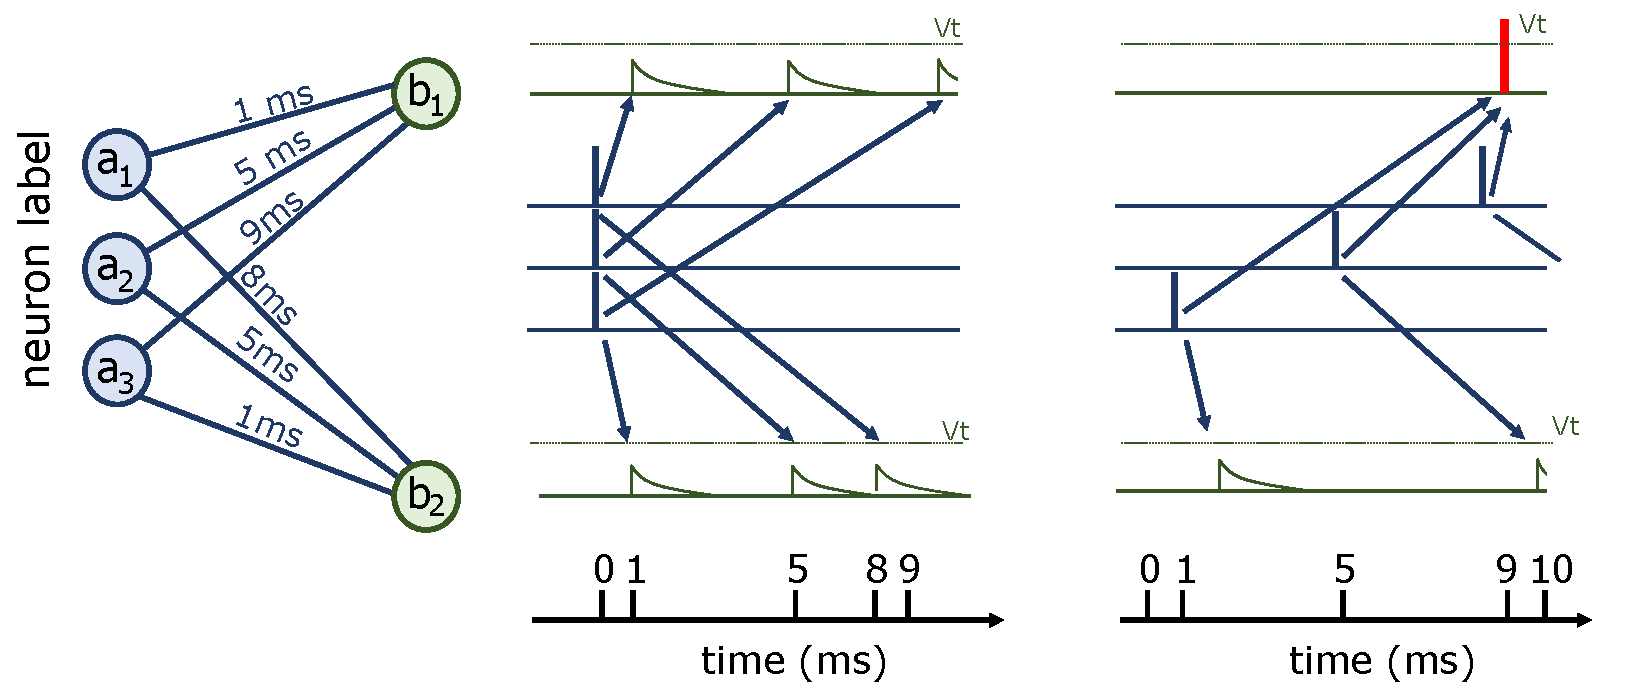
\includegraphics[width=0.98\linewidth]{figures/izhikevich.pdf}% https://www.overleaf.com/5625872443qpcwrkssgbsf
    \caption{
      \textbf{Core Mechanism of Spiking Motif Detection:}
      In this illustrative example, we consider a scenario involving three presynaptic neurons denoted as $a_1$, $a_2$, and $a_3$, which are fully connected to two postsynaptic neurons $b_1$ and $b_2$. The synaptic delays for the connections to $b_1$ are $1$, $5$, and $9~\ms$, while for $b_2$ they are $8$, $5$, and $1~\ms$, respectively.
      %
      In the middle panel, when the three presynaptic neurons emit synchronous pulses, the postsynaptic potentials generated in $b_1$ and $b_2$ reach them asynchronously due to the heterogeneous delays. Consequently, the postsynaptic potentials may not be sufficient to reach the membrane threshold (dashed line) in either of the postsynaptic neurons, and no output spike is generated.
      %
      In the right panel, the pulses emitted by the presynaptic neurons are arranged in such a way that, taking into account the delays, they reach the postsynaptic neuron $b_1$ at the same time (at $t=10~\ms$ in this example). As a result, the postsynaptic potentials $V_t$ evoked by the three presynaptic neurons sum up, causing the voltage threshold to be crossed. This leads to the emission of an output spike, signaling the detection of a spiking motif in the presynaptic population (highlighted in red color).
      %
      This core mechanism illustrates how the interplay between heterogeneous delays in the network allows for precise spike timing, enabling the detection of spiking motifs in neural populations. %Such precise spike timing is of potential significance in neural information processing and highlights how spiking motifs could play a crucial role in brain function.      
    }
  \label{fig:izhikevich}
\end{figure}
%----------------------------%
%
In recent studies, the importance of spike timing has been emphasized, especially in the barn owl auditory system, where precise spike timing in response to the sound of a mouse allows the brain to determine the prey's position~\cite{goodman_spike-timing-based_2010}. This discovery aligns with a growing body of literature suggesting that the brain's dynamics often exhibit stereotyped sequences known as \emph{spiking motifs}~\cite{grimaldi_precise_2023}. The concept of spiking motifs is a generalization of the patterns observed in the \textit{polychronization} model developed by Izhikevich~\cite{izhikevich_polychronization_2006}. This theoretical model comprises a random recurrent network of spiking neurons with biologically realistic synaptic delays and evolving weights governed by Spike-Time Dependent Plasticity (STDP) learning rule.

The interplay between the synaptic delays and STDP leads to the spontaneous organization of neurons into groups called "polychronous groups." Despite neurons in one of these groups firing at different times, the heterogeneous delays enable their spikes to converge synchronously on the postsynaptic neuron. This convergence results in the summation of excitatory postsynaptic potentials, leading to the firing of the postsynaptic neuron (see Figure~\ref{fig:izhikevich}). The polychronization model allows spiking neurons to self-organize into groups and generate reproducible time-locked spiking motifs. The STDP rule increases synaptic weights selectively for neurons involved in these polychronous groups, thereby consolidating the formation of such groups.

While the polychronization model provides valuable insights into understanding spiking neural networks and their potential role in generating spatio-temporal spiking motifs, it has a limitation. The model's heterogeneous delays are fixed and cannot evolve over time, which may limit its applicability in certain scenarios. However, the underlying mechanism offers valuable implications for studying neural activity motifs and their significance in the brain. To effectively detect spiking motifs, we propose a novel metric inspired by this model.
%%%%%%%%%%%%%%%%%%%%%%%%%%%%%%%%%%%%%%%%%%%%%
\subsection{The Heterogeneous Delays Spiking Neural Network (HD-SNN)}
%%%%%%%%%%%%%%%%%%%%%%%%%%%%%%%%%%%%%%%%%%%%%

In this work, we propose to accurately detect spatio-temporal spiking motifs using a feed-forward, single layer heterogeneous delays spiking neural network (HD-SNN). The paper is organized as follows. We develop a theoretically defined HD-SNN for which we can attune both the weights and delays. We first detail the methodology by defining the basic mechanism of spiking neurons that utilize heterogeneous delays. 
This will allow us to formalize the spiking neuron used to learn the model's parameters in a supervised manner and test its effectiveness. In the results section, we will first evaluate the efficiency of the learning scheme. We will also study the robustness of the spiking motif detection mechanism and in particular its resilience to changing the dimensions of the presynaptic or postsynaptic populations, or the depth in the number of different possible delays. Then, we will explore how the spiking motifs may be learned using supervised learning, and evaluate how the efficiency of the algorithm may depend on the parameters of the HD-SNN architecture. This will allow us to show how such a model can provide an efficient solution which may in the future be applied to neurobiological data.  Finally, we will conclude by highlighting the main contributions of this paper, while defining some limitations which will open perspectives for future detection methods. %In particular, as neuromorphic devices are by design good candidates for integrating computations over time, we highlight the fact that this event-driven algorithm is perfectly fit to be transferred to this type of hardware and to obtain significant gains in the energy which is used.
%
\section{Methods}
\label{sec:methods}
%%%-----------------------------------------------------------------
%%%-----------------------------------------------------------------
Let us formally define the HD-SNN model. First, we will define raster plots similar to those obtained from Single Unit Activity (SUA) recordings using an event-based and then binarized setting. We will then derive a generative model for raster plots using a HD-SNN, and derive a model for efficient detection of event-based motifs using a similar HD-SNN with ``inverted'' delays.
%
\subsection{Raster plots: from event-based to binarized}
%
In neurobiological recordings, %or in the sensory signal obtained from an event-based camera, 
any generic raster plot consists of a stream of \emph{spikes}. This can be formalized as a list of neural addresses and timestamps tuples $\event = \{(\presynaddr_\arank, \timev_\arank)\}_{\arank \in [1,\numevent]}$ where $\numevent \in \mathbb{N}$ is the total number of events in the data stream and the rank $\arank$ is the index of each event in the list of events. Each event has a time of occurrence $\timev_\arank$ (these are typically ordered) and an associated address $\presynaddr_\arank$ in the space $\presynaddrspace$ of the neural population. In a neurobiological recording like that of SUAs, this can be the identified set of neurons.

Events are generated by neurons which are defined on the one hand by the equations governing the evolution of its membrane potential dynamics on their soma and on the other hand by the integration of the synaptic potential propagating on their dendritic tree. A classical characterization consists in detailing the synaptic weights of each synaptic contact, the so-called weight matrix. As we saw above, neurons can receive inputs from multiple presynaptic neurons with heterogeneous delays. These delays represent the time it takes for a presynaptic spike to reach the soma of the postsynaptic neuron. 
%, and how this changes the network's dynamics~\cite{izhikevich_polychronization_2006}. 
In such neurons, %we can parameterize each neuron by the set of tuples defining both the weight and the delay of each synaptic contact. As a consequence, a set of 
input presynaptic spikes $\event$ will be multiplexed in time by the dendrites defined by this synaptic set (see Figure~\ref{fig:izhikevich}). %, and notably by the respective delays which will multiplex in time all events. 

Let's formalize such a layer of spiking neurons in the HD-SNN model. Each postsynaptic neuron $\postsynaddr \in \postsynaddrspace$  connects to presynaptic neurons from a set of addresses in  $\presynaddrspace$. In biology, a single cortical neuron has generally several thousands of synapses. Each may be defined by its synaptic weight and also its delay. %, that is, the time it takes for one spike to travel from the presynaptic neuron's soma to that of the postsynaptic neuron. %Neuron $\postsynaddr \in \postsynaddrspace$ is then described by the synaptic weights connecting it to a presynaptic afferent from $\presynaddrspace$ but also by the set of possible delays. 
Note that two neurons may contact with multiple synapses, and thus different delays. Scanning all neurons $\postsynaddr$, we thus define the set of $\Nsyn \in \mathbb{N}$ synapses  as  $\synapse = \{(\presynaddr_\ranksyn, \postsynaddr_\ranksyn, \synapticweight_\ranksyn, \synapticdelay_\ranksyn)\}_{\ranksyn \in [1,\Nsyn]}$, where each synapse is associated to a presynaptic address $\presynaddr_\ranksyn$, a postsynaptic address $\postsynaddr_\ranksyn$,  a weight $\synapticweight_\ranksyn$, and a delay $\synapticdelay_\ranksyn$. 

This defines the full connectivity of the HD-SNN model. The receptive field of a postsynaptic neuron refers to the set of synapses that connect to it. Similarly, the emitting field of a presynaptic neuron refers to the set of synapses it connects to. These fields determine the synaptic inputs and outputs of individual neurons. More formally, the receptive field of a postsynaptic neuron is defined $\synapse^\postsynaddr =  \{(\presynaddr_\ranksyn, \postsynaddr_\ranksyn, \synapticweight_\ranksyn, \synapticdelay_\ranksyn) \| \postsynaddr_\ranksyn=\postsynaddr\}_{\ranksyn \in [1,\Nsyn]} $, and the emitting field of a presynaptic neuron as $\synapse_\presynaddr =  \{(\presynaddr_\ranksyn, \postsynaddr_\ranksyn, \synapticweight_\ranksyn, \synapticdelay_\ranksyn) \| \presynaddr_\ranksyn=\presynaddr\}_{\ranksyn \in [1,\Nsyn]}$. Following this definition, an event stream which evokes neurons in the presynaptic address space is multiplexed by the synapses into a new event stream which is defined by the union of the sets generated by each emitting field from the presynaptic space: 
$ \cup_{\arank \in [1,\numevent]}  \{(\postsynaddr_\ranksyn, \synapticweight_\ranksyn, \timev_\arank + \synapticdelay_\ranksyn) \}_{ \ranksyn \in \synapse_{\presynaddr_\arank}} $. In biology, this new stream of events is naturally ordered in time as events reach the soma of post-synaptic neurons. %In particular, when post-synaptic neurons are activated on their soma by this spatio-temporal motif, the firing probability will increase, notably when these spikes converge on the soma in a synchronous manner. 
Synchronous activation of postsynaptic neurons, where multiple spikes converge on the soma simultaneously, will increase the firing probability of those neurons.

From the perspective of simulating such event-based computations on standard CPU- or GPU-based computers, it is useful to transform this event-based representation into a dense representation. Indeed, we may transform any event-based input as the boolean matrix $A \in \{0, 1 \}^{N\times T}$, where $N$ is the number of presynaptic neurons in $\presynaddrspace$ and $T$ is the number of time bins (see Figure~\ref{fig:THC}a). In this simplified model, we will consider that heterogeneous delays are integers limited in range between $0$ and $D$ (that is, $\forall {\ranksyn \in [1,\Nsyn]}$, $0 \le \synapticdelay_\ranksyn < D$) such that the synaptic set can be represented by the dense matrix $\kernel^\postsynaddr \in \mathbb{R}^{N\times D}$ giving for each neuron $\postsynaddr$ the weights as a function of presynaptic address and delay (see Figure~\ref{fig:THC}b). It is equal to zero except on synapses: $\forall {\ranksyn \in \synapse^\postsynaddr}, \kernel^\postsynaddr(\presynaddr_\ranksyn,  \synapticdelay_\ranksyn) = \synapticweight_\ranksyn$. Equivalently, one may define for each presynaptic neuron $\presynaddr$ the emitting kernel as the transpose kernel $\kernel^T_\presynaddr \in \mathbb{R}^{M\times D}$, where $M$ is the number of postsynaptic neurons, whose values are zero except on synapses:  $\forall {\ranksyn \in \synapse_\presynaddr}, \kernel^T_\presynaddr(\postsynaddr_\ranksyn,  \synapticdelay_\ranksyn) = \synapticweight_\ranksyn$.
%---------------------------
\begin{figure}%[t]%[h!]
% \begin{center}
  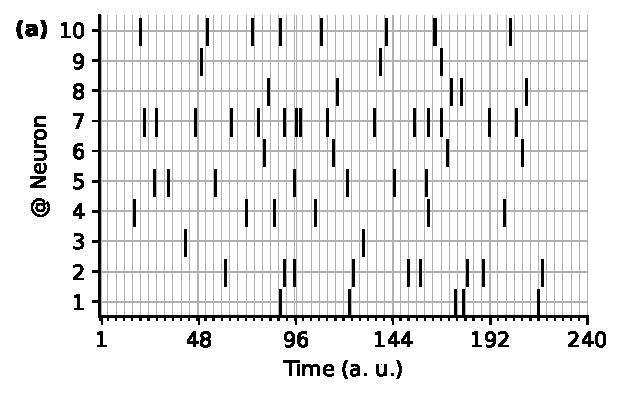
\includegraphics[width=.50\linewidth]{figures/THC_toy-a_k.pdf}
  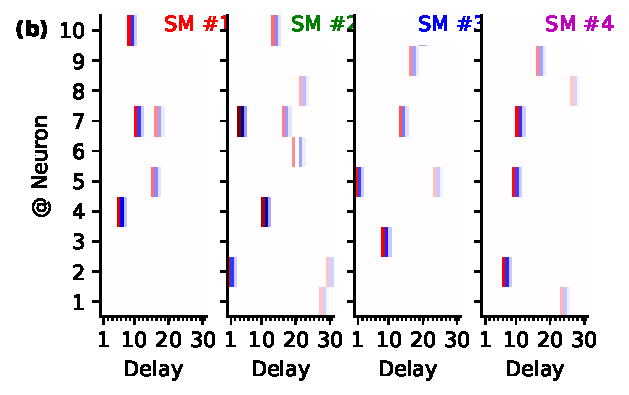
\includegraphics[width=.50\linewidth]{figures/THC_toy-b.pdf}
  \\
  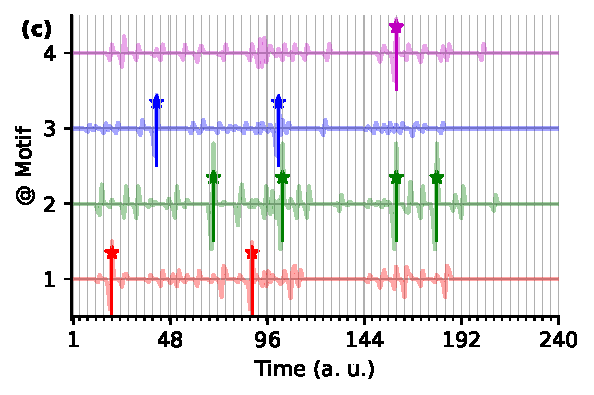
\includegraphics[width=.50\linewidth]{figures/THC_toy-c.pdf}
  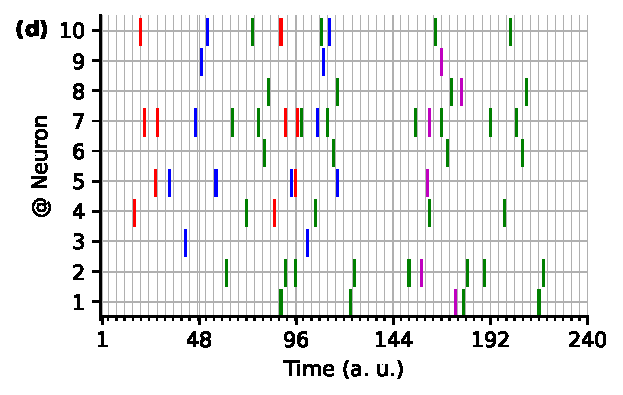
\includegraphics[width=.50\linewidth]{figures/THC_toy-a.pdf} 
% \end{center}
\caption{\textbf{From generating raster plots to inferring spiking motifs}. \textit{(a)}~As an illustration for the generative model, we draw a multiunit raster plot synthesized from $4$ different spiking motifs and for $10$ presynaptic neurons. \textit{(b)}~We show these motifs, each identified at the top by a different color. The evidence of activation (red) or deactivation (blue) is assigned to each presynaptic neuron and $31$ different possible delays. \textit{(c)}~The activation in time of the different motifs (denoted by stars) is drawn at random and then used to generate a raster plot on the multi-unit address space (see panel a). By inverting this model, an inference model can be defined for their efficient detection, outputting an evidence value (continuous line) from which the identity and timing of SMs can be inferred (vertical bars). \textit{(d)}~The original raster plot can be annotated with each identified spiking motif (as represented by the respective color assigned to SMs).
}
\label{fig:THC}
\end{figure}
%---------------------------
\subsection{A generative model for raster plots}

As described in Figure~\ref{fig:izhikevich}, a spiking motif can be detected using a properly tuned HD-SNN that maximizes spike synchronization at the postsynaptic terminal. Taking the argument the other way around, one may form a generative model for realistic raster plots in which spikes in the presynaptic address space are generated as the conjunction of spiking motifs defined in the postsynaptic space, knowing that both populations are connected by a set of weights and delays whose structure is stable relatively to the coding timescale. When connection weights are strong and sparsely distributed, this firing will robustly cause a specific temporal motif. Overall, these examples show that raster plots may be considered as a mixture of the effects of different elementary causes, and that each event triggers a specific spatio-temporal spiking motif. 

Formally, the activation of spiking motifs can occur independently and at random times. The activity is represented as a boolean matrix $B\in \{0, 1\}^{M\times T}$, where $M$ is the number of different spiking motifs (see Figure~\ref{fig:THC}c). Each entry $B(\postsynaddr, t)$ indicates whether a particular motif $\postsynaddr$ is activated at time $t$. The firing of a neuron $\presynaddr$ at time $t$ is considered a Bernoulli trial with a bias parameter $p(\presynaddr, t) \in [0, 1]$. This bias is conditioned by the presence of spiking motifs on postsynaptic neurons with corresponding delays. 
Assuming that this bias is conditioned by the presence of spiking motifs on \emph{all} efferent postsynaptic neurons with the corresponding delays, it can be shown that the logit (inverse of the sigmoid) of this probability bias can be written as the sum of the logit of each of these factors, whose values we will define as the corresponding weights in the kernel. We can thus write the probability bias $p(a, t)$ as the accumulated evidence given these factors as 
\begin{equation*}
p(\presynaddr, t) = \sigma\big(\kernel_\presynaddrspace(\presynaddr) + \sum_{\postsynaddr \in \synapse_\presynaddr, 0 \le \synapticdelay \le D} B(\postsynaddr, t+\synapticdelay) \cdot  \kernel_\presynaddr(\postsynaddr, \synapticdelay)  \big)  
\end{equation*}
where $\sigma$ is the sigmoid function. We will further assume that kernel's weights are balanced (their mean is zero) and that $\kernel_\presynaddrspace$ is a bias such that $\forall \presynaddr, t$, $\sigma(\kernel_\presynaddrspace(\presynaddr))$ is the average background firing rate. 

Finally, we obtain the raster plot $A\in \{0, 1\}^{N\times T}$ by drawing spikes using independent Bernoulli trials based on the computed probability biases $A \sim \mathcal{B}(p)$. Note that, depending on the definition of kernels, the generative model can model a discretized Poisson process, generate rhythmic activity or more generally propagating waves. This formulation thus defines a simple generative model for raster plots as a combination of independent spiking motifs.  This generative model can be easily extented to include a refractory period in order to ensure that there is a minimum time gap between successive action potentials, preventing them from overlapping. This temporal separation allows for discrete and well-defined neural signals, enabling accurate information processing and mitigating signal interference. The refractory period contributes to energy efficiency in neural systems and plays a crucial role in temporal coding by creating distinct time windows between successive spikes. 
%
\subsection{Detecting spiking motifs}
%: Detection model
% 
Assuming the spiking motifs (as defined by the kernel $\kernel$) are known, the generative model allows to determine an inference model for detecting sources $\hat{B}$ when observing a raster plot $A$. Indeed, by using this forward model, it is possible to estimate the likelihood $p(b, t)$ for the presence of a spiking motif of address $b$ and at time $t$ by using the transpose convolution operator. This consists in using the emitting field $\synapse_\presynaddr$ of presynaptic neurons in place of the receptive field $\synapse^\postsynaddr$ of postsynaptic neurons. It thus comes that when observing $A$, then one may infer the logit of the probability as the sum of evidences:
\begin{equation*}
  p(\postsynaddr, t) = \sigma\big(\kernel_\postsynaddrspace(b) + \sum_{\presynaddr \in \synapse^\postsynaddr,  0 \le \synapticdelay \le D} A(\presynaddr, t-\synapticdelay) \cdot \kernel^\postsynaddr(\presynaddr, \synapticdelay) \big)  
\end{equation*}
This also takes the form of a temporal convolution. This assumption holds as long as the kernels are uncorrelated, a condition which is met here numerically by choosing a relatively sparse set of synapses (approximately $1\%$ of active synapses). Finally, we compute $\hat{B}$ by selecting the most likely items, allowing to identify the spiking motifs in the input raster plot (see Figure~\ref{fig:THC}d). 

One may naturally extend this algorithm when the spiking motifs (that is, the weights) are not known, but that we know the timing and identity of the spiking motifs. Indeed, the equation above is differentiable. Indeed, the activation function of our spiking neural is a sigmoid function implementing a form of  Multinomial Logistic Regression (MLR)~\cite{grimaldi_learning_2023}.  
The underlying metric is the binary cross-entropy, as used in the logistic regression model. In particular, if we consider kernels with similar decreasing exponential time profile, one can prove that this detection model is similar to the method of Berens {\it et al.}~\cite{berens_fast_2012}. In our specific case, the difference is that the regression is performed in both dendritic and delay space by extending the summation using a temporal convolution operator. 
% 
\section{Results}
%
To quantify the efficiency of this operation, we generated raster plots parameterized by $N=128$ presynaptic inputs and $M=144$ synthetic spiking motifs as random independent kernels and with $D=31$ possible delays. We drew random independent instances of $B$ with a length of $T=1000$ time steps and an average of $1.0$ spikes per neuron. This allowed us to generate a large number of synthetic raster plots, which we use to infer $\hat{B}$. We compute accuracy as the rate of true positive detections (both for inferring the address and its exact timing) and observe on average $\approx 98.8\%$ correct detections.

We extended this result by showing how accuracy evolves as a function of the number of simultaneous spiking motifs, holding the frequency of occurrence constant. We show in \fig{model_results}~(left) that the accuracy of finding the right spiking motif is still above $80\%$ accuracy with more than $1364$ overlapping spiking motifs. This observation illustrates quantitatively the capacity  of the HD-SNN in representing a high number of simultaneous motifs. Furthermore, we show in \fig{model_results}~(middle) that (with $M=144$ spiking motifs fixed) the accuracy increases significantly with increasing temporal depth $D$ of the spiking motif kernel, quantitatively demonstrating the computational advantage of using heterogeneous delays. These results were obtained under the assumption that we know the spiking motifs through $\kernel$. However, this is generally not the case, for example, when considering the raster plot of biological neurons.

Finally, we evaluated the performance of the supervised learning scheme in inferring the connection kernel when the address and timing of spiking motifs are known. The kernel was initialized with random independent values, and we used stochastic gradient descent with a learning rate of \num{1e-4} over $\num{1e4}$ trials (i.e., over rasters as defined above with $T=1000$ and $N=128$). Qualitatively, the convergence was monotonous, and the correct values of the $M=144$ spiking motifs were quickly recovered. Quantitatively, the correlation between the true and learned kernel weights showed that all kernels were correctly recovered (see Figure~\ref{fig:model_results}, right). Performing inference with the learned weights was as efficient as with the true kernels, and showed no significant difference (not shown).

%---------------------------
\begin{figure}%[t!]
  \centering
  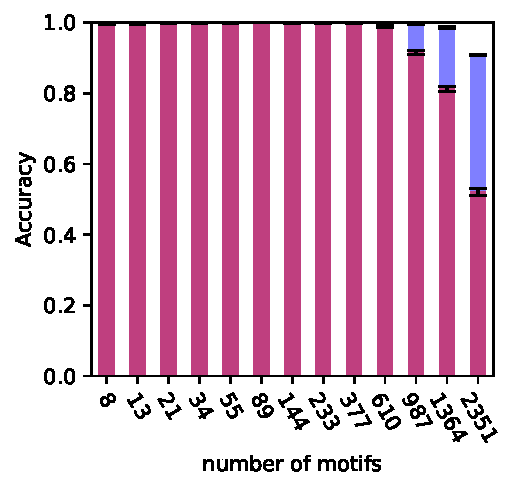
\includegraphics[width=0.335\linewidth]{figures/THC_N_SMs.pdf}
  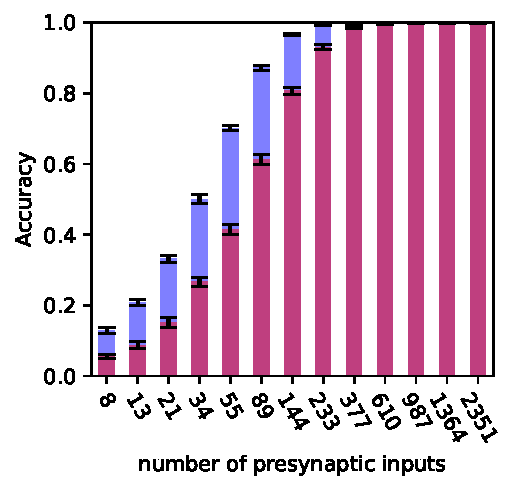
\includegraphics[width=0.320\linewidth]{figures/THC_N_pre.pdf}
  % 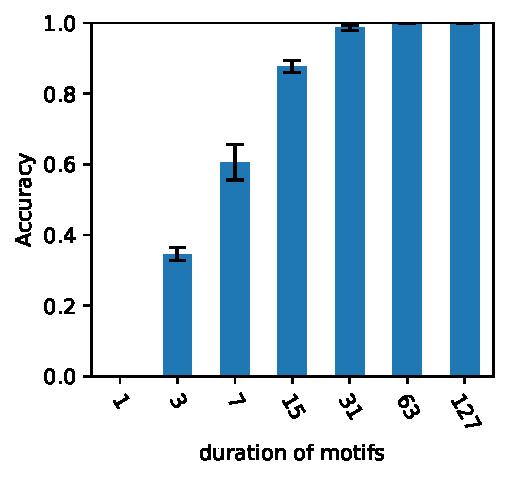
\includegraphics[width=0.330\linewidth]{figures/THC_N_SM_time.pdf} 
  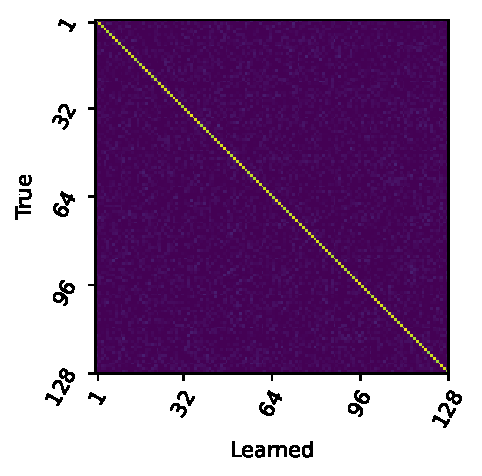
\includegraphics[width=0.315\linewidth]{figures/THC_xcorr-supervised.pdf}
    \caption{{\bf Detecting spiking motifs using spiking neurons with heterogeneous delays.} 
Accuracy of detection for the classical correlation (red) and the HD-SNN method (blue) as a function of  {\it (Left)}~the number $M$ of kernels, 
    {\it (Middle)}~the number of presynaptic neurons, 
    % {\bf (Middle)}~the temporal depth $D$ of kernels among $M=144$ kernels.
    {\it (Right)} Correlation matrix of true vs learned kernels.
    }
  \label{fig:model_results}
\end{figure}
%---------------------------
%
\section{Discussion}
%
\subsection{Synthesis and Main Contributions}
%%%-----------------------------------------------------------------
In this paper, we present a novel Heterogeneous Delays Spiking Neural Network (HD-SNN) model designed for the detection of spiking motifs in synthetic neurobiologically-inspired raster plots.

Our contributions encompass several innovations. Firstly, we formulate the HD-SNN model from first principles, optimizing the detection of event-based spatiotemporal motifs. Unlike previous models like the tempotron, which are evaluated on simplified problems, our model is rigorously tested on realistic synthetic data. The results demonstrate that, assuming that the spiking motifs are known, our model accurately detects the identity and timing of spiking motifs, even when multiple motifs are superimposed. Additionally, we show that our method outperforms correlation-based heuristics, such as those used in previous works like~\cite{ghosh_spatiotemporal_2019,yu_stsc-snn_2022}, in terms of efficiency. Secondly, compared to other event-based methods, like HOTS~\cite{lagorce_hots_2017}, our model's weights are interpretable. These weights are directly related to the logit, which is the inverse sigmoid of the probability of detecting each spatiotemporal spiking motif. Finally, a crucial novelty lies in the simultaneous learning of weights and delays in our model. In contrast, models like the polychronization model~\cite{izhikevich_polychronization_2006} only learn weights and delays are frozen. These contributions highlight the significance and effectiveness of our HD-SNN model for detecting spiking motifs, offering insights into the neural mechanisms involved in pattern recognition and information processing.

\subsection{Main limits}
%%%----------------------------------------------------------------- %

The model comes with certain limitations. First, the entire framework is based on discrete time binning, which is incompatible with the continuous nature of biological time. While this choice facilitated efficient implementation on conventional hardware such as GPUs, it can be extended to a purely event-based SNN framework~\cite{grimaldi_robust_2023}. By analytically incorporating a precision term in the temporal value of the input spikes, a purely event-based scheme can be achieved, promising speedups and computational energy gains.

Second, the current model is purely feed-forward, i.e. the spikes generated by postsynaptic neurons are based solely on information from their classical receptive fields. However, neural systems often involve lateral interactions between neurons in the same layer and feedback connections, which can be crucial for computational principles and modulation of neural information. While our theoretical model can incorporate these recurrent connections by inserting new spikes into the list of spikes reaching presynaptic addresses, it requires proper tuning to avoid perturbations of the homeostatic state. For the implementation of predictive or anticipatory processes, recurrent activity would be essential, especially when dealing with multiple different delays that require temporal alignment. Such recurrent activity has previously been modelled to explain phenomena such as the flash-lag illusion. Implementing this using generalised coordinate and delay operators would allow predictive mechanisms to be incorporated into our proposed HD-SNN model, providing an elegant solution to this problem.

Addressing these limitations and exploring the extension of the HD-SNN model to event-based schemes and recurrent connections would enrich its potential applications and pave the way for a better understanding of neural information processing in complex systems.
%
\subsection{Perspectives}
%%%-----------------------------------------------------------------
% learning
The coding results were obtained under the assumption that we know the spiking motifs by way of $\kernel$, or using supervised learning by knowing the identity and timing of spiking motifs. However, this is generally not the case, e.g. when observing the neurobiological raster plot of a population of neurons. One perspective would be to extend the model to a fully self-supervised learning paradigm, i.e. without any labeled data~\cite{barlow_unsupervised_1989}. This type of learning is thought to be prevalent in the central nervous system and, assuming the signal is sparse~\cite{olshausen_emergence_1996}, one could extend these Hebbian sparse learning schemes to spikes~\cite{perrinet_emergence_2004,masquelier_competitive_2009}. 

We expect that this would be particularly adapted for exploring neurobiological data~\cite{mackevicius_unsupervised_2019}. Indeed, there is a large literature showing that brain dynamics often organize into stereotyped sequences such as synfire chains~\cite{ikegaya_synfire_2004}, packets~\cite{luczak_sequential_2007}, or hippocampal sequences~\cite{villette_internally_2015} (for a review, see~\cite{grimaldi_precise_2023}). These motifs are stereotyped and robust, as they can be activated in the same motif from day to day~\cite{haimerl_internal_2019}. In contrast to conventional methods used to process neurobiological data, such an event-based model would be able to answer key questions regarding the representation of information in neurobiological data. %Furthermore, it would open possibilities in the field of machine learning, especially in computer vision, to address current key concerns such as robustness to attacks, scalability, interpretability, or energy consumption.
% However, there is no ground truth and one needs to develop a self-supervised learning algorithm for the automatic detection of spiking motifs, a challenging fior the future of our understanding of neurobiological data. 
%Inspired by the k-means algorithm,For this, we can initialize $\kernel$ at random and define an auto-encoder scheme that infers the sources $\hat{B}$ for each input $A$ and then resynthesizes the corresponding raster plot. %A natural metric is again binary cross-entropy, as used in the logistic regression model. Since the model is differentiable, we can optimize $\kernel$ using gradient descent. We can add a homeostatic regularization on the average firing rate of $B$ to ensure that each motif was \emph{a priori} equally activated~\cite{perrinet_adaptive_2019}. Our preliminary results show that it is possible to retrieve spiking motifs embedded in synthetic data. However, further analysis is needed to improve the convergence of the algorithm and to apply such algorithms to real neurobiological data.  In particular, it seems promising to use a sparseness constraint in the inference mechanism to remove spurious correlations in the inference.
%
% \bibliographystyle{splncs04}
% %
% \bibliography{polychronies}
% % 
\begin{thebibliography}{10}
  \providecommand{\url}[1]{\texttt{#1}}
  \providecommand{\urlprefix}{URL }
  \providecommand{\doi}[1]{https://doi.org/#1}
  
  \bibitem{barlow_unsupervised_1989}
  Barlow, H.: Unsupervised {Learning}. Neural Computation  \textbf{1}(3),  295--311 (Sep 1989). %\doi{10.1162/neco.1989.1.3.295}, \url{https://doi.org/10.1162/neco.1989.1.3.295}, 00000
  
  \bibitem{berens_fast_2012}
  Berens, P., Ecker, A.S., Cotton, R.J., Ma, W.J., Bethge, M., Tolias, A.S.: A {Fast} and {Simple} {Population} {Code} for {Orientation} in {Primate} {V1}. Journal of Neuroscience  \textbf{32}(31),  10618--10626 (2012). %\doi{10.1523/jneurosci.1335-12.2012}, \url{https://doi.org/f365rn}
  
  \bibitem{boutin_sparse_2020}
  Boutin, V., Franciosini, A., Chavane, F.Y., Ruffier, F., Perrinet, L.U.: Sparse {Deep} {Predictive} {Coding} captures contour integration capabilities of the early visual system. PLoS Computational Biology  (May 2020). % \doi{10.1371/journal.pcbi.1008629}, \url{https://doi.org/10.1371/journal.pcbi.1008629}, tex.date-added: 2019-06-18 13:53:53 +0200 tex.date-modified: 2020-12-12 11:55:20 +0100 tex.grants: doc-2-amu,phd-icn,mesocentre tex.preprint: https://arxiv.org/abs/1902.07651 tex.url\_code: https://github.com/VictorBoutin/InteractionMap publisher: Public Library of Science San Francisco, CA USA
  
  \bibitem{boutin_effect_2020}
  Boutin, V., Franciosini, A., Ruffier, F., Perrinet, L.U.: Effect of top-down connections in {Hierarchical} {Sparse} {Coding}. Neural Computation  \textbf{32}(11),  2279--2309 (Feb 2020). % \doi{10.1162/neco_a_01325}, \url{https://laurentperrinet.github.io/publication/boutin-franciosini-ruffier-perrinet-20-feedback/}, tex.ids= BoutinFranciosiniRuffierPerrinet20 tex.date-modified: 2020-11-03 09:59:57 +0100 tex.grants: doc-2-amu,phd-icn,mesocentre tex.preprint: https://arxiv.org/abs/2002.00892 publisher: MIT Press
  
  \bibitem{chavane_revisiting_2022}
  Chavane, F., Perrinet, L.U., Rankin, J.: Revisiting horizontal connectivity rules in {V1}: from like-to-like towards like-to-all. Brain Structure and Function  (Feb 2022). % \doi{10.1007/s00429-022-02455-4}, \url{https://doi.org/10.1007/s00429-022-02455-4}
  
  \bibitem{ghosh_spatiotemporal_2019}
  Ghosh, R., Gupta, A., Silva, A.N., Soares, A., Thakor, N.V.: Spatiotemporal filtering for event-based action recognition (2019). %, \url{http://arxiv.org/abs/1903.07067}
  
  \bibitem{goodman_spike-timing-based_2010}
  Goodman, D.F.M., Brette, R.: Spike-timing-based computation in sound localization. PLoS Comput Biol  \textbf{6}(11) (Nov 2010). % \doi{10.1371/journal.pcbi.1000993}, \url{http://www.ncbi.nlm.nih.gov/pmc/articles/PMC2978676/}
  
  \bibitem{grimaldi_robust_2023}
  Grimaldi, A., Boutin, V., Ieng, S.H., Benosman, R., Perrinet, L.U.: A robust event-driven approach to always-on object recognition. Neural Networks  (2023). % \doi{https://laurentperrinet.github.io/publication/grimaldi-23/}
  
  \bibitem{grimaldi_precise_2023}
  Grimaldi, A., Gruel, A., Besnainou, C., Jérémie, J.N., Martinet, J., Perrinet, L.U.: Precise {Spiking} {Motifs} in {Neurobiological} and {Neuromorphic} {Data}. Brain Sciences  \textbf{13}(1), ~68 (Jan 2023). % \doi{10.3390/brainsci13010068}, \url{https://www.mdpi.com/2076-3425/13/1/68}, number: 1 Publisher: Multidisciplinary Digital Publishing Institute
  
  \bibitem{grimaldi_learning_2023}
  Grimaldi, A., Perrinet, L.U.: Learning heterogeneous delays in a layer of spiking neurons for fast motion detection. Biological Cybernetics  (Jun 2023). %, \url{https://laurentperrinet.github.io/publication/grimaldi-23-bc/}
  
  \bibitem{grun_unitary_2002-1}
  Grün, S., Diesmann, M., Aertsen, A.: Unitary {Events} in {Multiple} {Single}-{Neuron} {Spiking} {Activity}: {II}. {Nonstationary} {Data}. Neural Computation  \textbf{14}(1),  81--119 (Jan 2002). % \doi{10.1162/089976602753284464}, \url{https://doi.org/ffvbkp}
  
  \bibitem{gutig_tempotron_2006}
  Gütig, R., Sompolinsky, H.: The tempotron: a neuron that learns spike timing–based decisions. Nature Neuroscience  \textbf{9}(3),  420--428 (2006). % \doi{10.1038/nn1643}, \url{https://doi.org/ch29r4}
  
  \bibitem{haimerl_internal_2019}
  Haimerl, C., Angulo-Garcia, D., Villette, V., Reichinnek, S., Torcini, A., Cossart, R., Malvache, A.: Internal representation of hippocampal neuronal population spans a time-distance continuum. Proceedings of the National Academy of Sciences  \textbf{116}(15),  7477--7482 (Apr 2019). % \doi{10.1073/pnas.1718518116}, \url{https://www.pnas.org/content/116/15/7477}
  
  \bibitem{hogendoorn_predictive_2019}
  Hogendoorn, H., Burkitt, A.N.: Predictive {Coding} with {Neural} {Transmission} {Delays}: {A} {Real}-{Time} {Temporal} {Alignment} {Hypothesis}. eneuro  \textbf{6}(2),  ENEURO.0412--18.2019 (Mar 2019). % \doi{10.1523/eneuro.0412-18.2019}, \url{http://eneuro.org/lookup/doi/10.1523/ENEURO.0412-18.2019}
  
  \bibitem{ikegaya_synfire_2004}
  Ikegaya, Y., Aaron, G., Cossart, R., Aronov, D., Lampl, I., Ferster, D., Yuste, R.: Synfire {Chains} and {Cortical} {Songs}: {Temporal} {Modules} of {Cortical} {Activity}. Science  \textbf{304}(5670),  559--564 (Apr 2004). % \doi{10/djckcn}, \url{http://www.science.org/doi/10.1126/science.1093173}
  
  \bibitem{izhikevich_polychronization_2006}
  Izhikevich, E.M.: Polychronization: {Computation} with {Spikes}. Neural Computation  \textbf{18}(2),  245--282 (Feb 2006). % \doi{10/bgh4qv}, \url{https://doi.org/10.1162/089976606775093882}, 00000
  
  \bibitem{khoei_flash-lag_2017}
  Khoei, M.A., Masson, G.S., Perrinet, L.U.: The {Flash}-{Lag} {Effect} as a {Motion}-{Based} {Predictive} {Shift}. PLOS Computational Biology  \textbf{13}(1),  e1005068 (Jan 2017). % \doi{10.1371/journal.pcbi.1005068}, \url{https://journals.plos.org/ploscompbiol/article?id=10.1371/journal.pcbi.1005068}, publisher: Public Library of Science
  
  \bibitem{lagorce_hots_2017}
  Lagorce, X., Orchard, G., Galluppi, F., Shi, B.E., Benosman, R.B.: {HOTS}: {A} {Hierarchy} of {Event}-{Based} {Time}-{Surfaces} for {Pattern} {Recognition}. IEEE Transactions on Pattern Analysis and Machine Intelligence  \textbf{39}(7),  1346--1359 (2017). % \doi{10.1109/TPAMI.2016.2574707}, \url{http://www.ncbi.nlm.nih.gov/pubmed/27411216%20http://ieeexplore.ieee.org/document/7508476/}
  
  \bibitem{levakova_review_2015}
  Levakova, M., Tamborrino, M., Ditlevsen, S., Lansky, P.: A review of the methods for neuronal response latency estimation. Biosystems  \textbf{136},  23--34 (Oct 2015). % \doi{10.1016/j.biosystems.2015.04.008}, \url{https://doi.org/gpshjz}
  
  \bibitem{luczak_sequential_2007}
  Luczak, A., Barthó, P., Marguet, S.L., Buzsáki, G., Harris, K.D.: Sequential structure of neocortical spontaneous activity in vivo. Proceedings of the National Academy of Sciences  \textbf{104}(1),  347--352 (Jan 2007). % \doi{10.1073/pnas.0605643104}, \url{https://www.pnas.org/content/104/1/347}
  
  \bibitem{mackevicius_unsupervised_2019}
  Mackevicius, E.L., Bahle, A.H., Williams, A.H., Gu, S., Denisenko, N.I., Goldman, M.S., Fee, M.S.: Unsupervised discovery of temporal sequences in high-dimensional datasets, with applications to neuroscience. eLife  \textbf{8},  e38471 (Feb 2019). % \doi{10.7554/eLife.38471}, \url{https://doi.org/10.7554/eLife.38471}, publisher: eLife Sciences Publications, Ltd
  
  \bibitem{masquelier_competitive_2009}
  Masquelier, T., Guyonneau, R., Thorpe, S.J.: Competitive {STDP}-{Based} {Spike} {Pattern} {Learning}. Neural Computation  \textbf{21}(5),  1259--1276 (May 2009). % \doi{10.1162/neco.2008.06-08-804}, \url{http://www.mitpressjournals.org/doi/10.1162/neco.2008.06-08-804}, 00203
  
  \bibitem{olshausen_emergence_1996}
  Olshausen, B.A., Field, D.J.: Emergence of simple-cell receptive field properties by learning a sparse code for natural images. Nature  \textbf{381}(6583),  607--609 (1996). % \doi{10.1038/381607a0}, \url{http://dx.doi.org/10.1038/381607a0 http://www.ncbi.nlm.nih.gov/htbin-post/Entrez/query?db=m&form=6&dopt=r&uid=8637596 http://www.ncbi.nlm.nih.gov/pubmed/8637596 http://www.nature.com/doifinder/10.1038/381607a0}, 00000
  
  \bibitem{pachitariu_robustness_2018}
  Pachitariu, M., Stringer, C., Harris, K.D.: Robustness of {Spike} {Deconvolution} for {Neuronal} {Calcium} {Imaging}. The Journal of Neuroscience  \textbf{38}(37),  7976--7985 (2018). % \doi{10.1523/jneurosci.3339-17.2018}, \url{https://doi.org/gd9mcx}
  
  % \bibitem{pastalkova_internally_2008}
  % Pastalkova, E., Itskov, V., Amarasingham, A., Buzsáki, G.: Internally {Generated} {Cell} {Assembly} {Sequences} in the {Rat} {Hippocampus}. Science (New York, N.Y.)  \textbf{321}(5894),  1322--1327 (Sep 2008). % \doi{10.1126/science.1159775}, \url{https://www.ncbi.nlm.nih.gov/pmc/articles/PMC2570043/}
  
  \bibitem{perrinet_emergence_2004}
  Perrinet, L.: Emergence of filters from natural scenes in a sparse spike coding scheme. Neurocomputing  \textbf{58-60}(C),  821--826 (2004). % \doi{10.1016/j.neucom.2004.01.133}, \url{http://linkinghub.elsevier.com/retrieve/pii/S0925231204001389}, tex.ids: Perrinet03 tex.date-modified: 2019-02-22 11:55:28 +0100
  
  \bibitem{perrinet_active_2014}
  Perrinet, L.U., Adams, R.A., Friston, K.J.: Active inference, eye movements and oculomotor delays. Biological Cybernetics  \textbf{108}(6),  777--801 (Dec 2014). % \doi{10.1007/s00422-014-0620-8}, \url{https://doi.org/10.1007/s00422-014-0620-8}
  
  % \bibitem{roelfsema_early_2016}
  % Roelfsema, P.R., de~Lange, F.P.: Early visual cortex as a multiscale cognitive blackboard. Annual review of vision science  \textbf{2},  131--151 (2016). % \doi{10.1146/annurev-vision-111815-114443}, publisher: Annual Reviews
  
  \bibitem{van_rossum_novel_2001}
  van Rossum, M.: A novel spike distance. Neural Comp  \textbf{13}(4),  751--763 (2001). % \doi{10.1162/089976601300014321}
  
  \bibitem{sotomayor-gomez_spikeship_2021}
  Sotomayor-Gómez, B., Battaglia, F.P., Vinck, M.: {SpikeShip}: {A} method for fast, unsupervised discovery of high-dimensional neural spiking patterns. bioRxiv : the preprint server for biology pp. 2020--06 (2021). % \doi{10.1101/2020.06.03.131573}, \url{https://www.biorxiv.org/content/10.1101/2020.06.03.131573}, publisher: Cold Spring Harbor Laboratory
  
  % \bibitem{stella_comparing_2022}
  % Stella, A., Bouss, P., Palm, G., Grün, S.: Comparing {Surrogates} to {Evaluate} {Precisely} {Timed} {Higher}-{Order} {Spike} {Correlations}. eneuro  \textbf{9}(3),  ENEURO.0505--21.2022 (2022). % \doi{10.1523/eneuro.0505-21.2022}, \url{https://doi.org/gqjvht}
  
  \bibitem{stella_3d-spade_2019}
  Stella, A., Quaglio, P., Torre, E., Grün, S.: 3d-{SPADE}: {Significance} evaluation of spatio-temporal patterns of various temporal extents. Biosystems  \textbf{185},  104022 (Nov 2019). % \doi{10.1016/j.biosystems.2019.104022}, \url{https://doi.org/gpshj2}
  
  \bibitem{victor_nature_1996}
  Victor, J.D., Purpura, K.P.: Nature and precision of temporal coding in visual cortex: a metric-space analysis. Journal of Neurophysiology  \textbf{76}(2),  1310--1326 (1996). % \doi{10.1152/jn.1996.76.2.1310}, \url{https://www.physiology.org/doi/10.1152/jn.1996.76.2.1310}
  
  \bibitem{villette_internally_2015}
  Villette, V., Malvache, A., Tressard, T., Dupuy, N., Cossart, R.: Internally {Recurring} {Hippocampal} {Sequences} as a {Population} {Template} of {Spatiotemporal} {Information}. Neuron  \textbf{88}(2),  357--366 (Oct 2015). % \doi{10/f7whnn}, \url{https://www.sciencedirect.com/science/article/pii/S0896627315008417}, 00085
  
  \bibitem{williams_point_2020}
  Williams, A.H., Degleris, A., Wang, Y., Linderman, S.W.: Point process models for sequence detection in high-dimensional neural spike trains. Tech. Rep. 2010.04875, arXiv (Oct 2020). %, \url{https://arxiv.org/abs/2010.04875}
  
  \bibitem{yu_stsc-snn_2022}
  Yu, C., Gu, Z., Li, D., Wang, G., Wang, A., Li, E.: {STSC}-{SNN}: {Spatio}-{Temporal} {Synaptic} {Connection} with {Temporal} {Convolution} and {Attention} for {Spiking} {Neural} {Networks} (Oct 2022), arXiv:2210.05241 % , \url{http://arxiv.org/abs/2210.05241}[cs, q-bio, stat]
  
  \end{thebibliography}
  
\end{document}
 